\documentclass[tikz,border=12pt]{standalone}
\usepackage{amsmath}
\usepackage{amssymb}
\usepackage{tikz}
\usetikzlibrary{arrows.meta}

\definecolor{ink}{HTML}{0F172A}
\definecolor{linegray}{HTML}{64748B}
\definecolor{visible}{HTML}{E2E8F0}
\definecolor{masked}{HTML}{F8FAFC}
\definecolor{reconstructed}{HTML}{CBD5E1}

\begin{document}
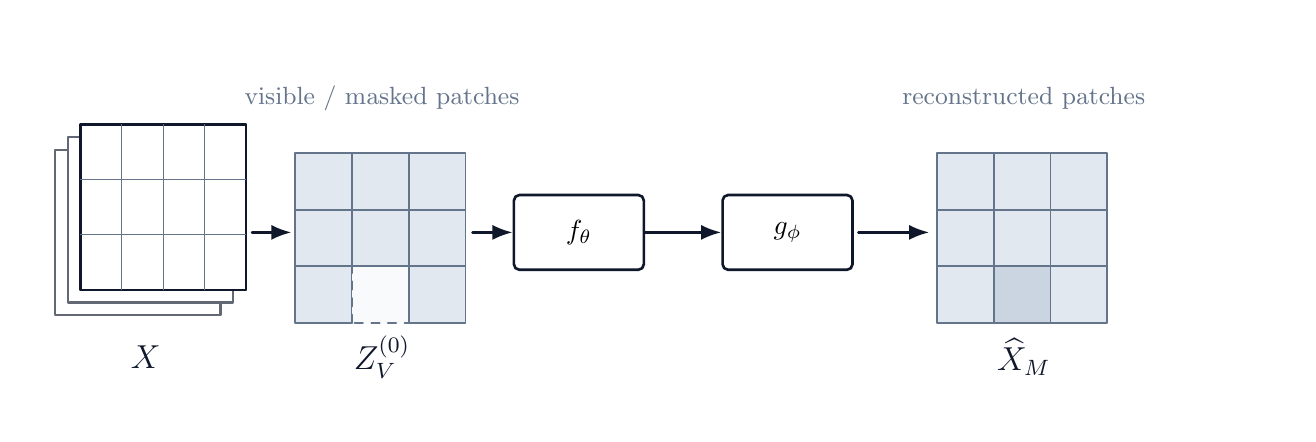
\begin{tikzpicture}[
  font=\sffamily,
  >=Latex,
  line cap=round,
  line join=round
]
  \fill[white] (0,0) rectangle (16,4.9);

  % Input: a stack of 2D image planes.
  \foreach \layer in {0,...,2} {
    \begin{scope}[xshift=0.16*\layer cm,yshift=0.16*\layer cm]
      \draw[ink!65, line width=0.85pt, fill=white] (0.35,1.25) rectangle (2.45,3.35);
    \end{scope}
  }
  \begin{scope}[xshift=0.32cm,yshift=0.32cm]
    \draw[ink, line width=0.85pt] (0.35,1.25) rectangle (2.45,3.35);
    \foreach \column in {0.875,1.4,1.925} {
      \draw[linegray, line width=0.35pt] (\column,1.25) -- (\column,3.35);
    }
    \foreach \row in {1.95,2.65} {
      \draw[linegray, line width=0.35pt] (0.35,\row) -- (2.45,\row);
    }
  \end{scope}
  \node[ink, font=\large] at (1.5,0.72) {$X$};

  % Patch grid: shaded cells are visible and dashed cells are masked.
  \begin{scope}[xshift=3.4cm,yshift=1.15cm]
    \foreach \row in {0,1,2} {
      \foreach \column in {0,1,2} {
        \pgfmathtruncatemacro{\cell}{3*\row+\column}
        \ifnum\cell=1
          \fill[masked] (\column*0.72,\row*0.72) rectangle ++(0.72,0.72);
          \draw[linegray, dashed, line width=0.7pt]
            (\column*0.72,\row*0.72) rectangle ++(0.72,0.72);
        \else
          \fill[visible] (\column*0.72,\row*0.72) rectangle ++(0.72,0.72);
          \draw[linegray, line width=0.7pt]
            (\column*0.72,\row*0.72) rectangle ++(0.72,0.72);
        \fi
      }
    }
  \end{scope}
  \node[ink, font=\large] at (4.5,0.72) {$Z_V^{(0)}$};
  \node[linegray, font=\small] at (4.5,4.0) {visible / masked patches};

  \draw[ink, ->, line width=0.95pt] (2.85,2.3) -- (3.35,2.3);

  % Encoder and decoder blocks.
  \node[draw=ink, line width=0.95pt, rounded corners=2pt,
    minimum width=1.65cm, minimum height=0.95cm, inner sep=2pt, fill=white]
    (encoder) at (7.0,2.3) {$f_\theta$};
  \node[draw=ink, line width=0.95pt, rounded corners=2pt,
    minimum width=1.65cm, minimum height=0.95cm, inner sep=2pt, fill=white]
    (decoder) at (9.65,2.3) {$g_\phi$};
  \draw[ink, ->, line width=0.95pt] (5.65,2.3) -- (encoder.west);
  \draw[ink, ->, line width=0.95pt] (encoder.east) -- (decoder.west);

  % Output: the masked patches are reconstructed.
  \begin{scope}[xshift=11.55cm,yshift=1.15cm]
    \foreach \row in {0,1,2} {
      \foreach \column in {0,1,2} {
        \pgfmathtruncatemacro{\cell}{3*\row+\column}
        \ifnum\cell=1
          \fill[reconstructed] (\column*0.72,\row*0.72) rectangle ++(0.72,0.72);
        \else
          \fill[visible] (\column*0.72,\row*0.72) rectangle ++(0.72,0.72);
        \fi
        \draw[linegray, line width=0.7pt]
          (\column*0.72,\row*0.72) rectangle ++(0.72,0.72);
      }
    }
  \end{scope}
  \draw[ink, ->, line width=0.95pt] (10.55,2.3) -- (11.45,2.3);
  \node[ink, font=\large] at (12.65,0.72) {$\widehat{X}_M$};
  \node[linegray, font=\small] at (12.65,4.0) {reconstructed patches};
\end{tikzpicture}
\end{document}
